%------------------------------------------------------------
%------------------------------------------------------------
\section{Introduction}
\label{sec:introduction}

Course and exam organization in universities involves strategic, tactical and operational decisions relating to curriculum design, student sectioning, course staffing, room planning, class scheduling and resource allocation \cite{2019_lindahl_EJOR}. 
These computational tasks and their overall coordination vary between countries and educational institutions as does the level of process automation and decision tool support \cite{2019_oude_AOR}. 
In French universities for instance  (see Figure~\ref{fig:utp-workflow}), curricula are conventionally revisited every 5 years and students enroll in courses prior to each teaching period in the course of the academic year. Demand is matched by sectioning courses into classes, partitioning students into fixed groups, and populating classes with groups. Eligible groups, lecturers, rooms and equipment are then identified for each course before class sessions get scheduled and allocated the necessary resources. 
Each stage involves different stakeholders with their own requirements (faculty departments, administrative units, course owners, lecturers, tutors, etc.) and the workflow naturally allows for deviations and contingencies (marginal amendments to curricula on a yearly basis, late student registrations, staff absences, etc.).

\begin{figure}[h]
\begin{center}
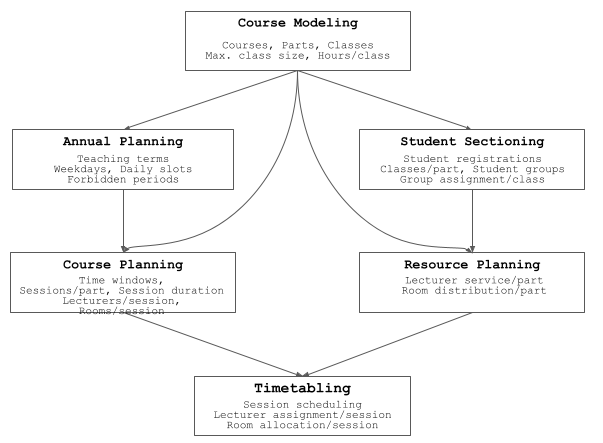
\includegraphics[scale=0.4]{img/utp_workflow.png}
\end{center}
\caption{Conventional workflow for course organization in French universities.}%: steps and roles}
\label{fig:utp-workflow}
\end{figure}

%The scope of these computational tasks and the overall workflow vary between countries and educational institutions as does the level of process automation and decision tool support \cite{2019oudevrielinkAOR}. 
Various problem formulations together with data formats and algorithms 
have been proposed in the literature to tackle specific aspects of university timetabling including 
curriculum balancing %for assigning courses to teaching termes while balancing student workload 
\cite{2001_castro_ARXIV,2012_chiarandini_JH,2013_rubio_MPE}, 
student sectioning \cite{2010_muller_AOR,2019_schindl_AOR}, 
%(strategic) room planning {2017lindhalEJOR}, 
examination timetabling \cite{1996_carter_JORS,2020_battistutta_CPAIOR,2010_mccollum_INFORMS},
curriculum-based %course timetabling \cite{2010mccollumINFORMS,2015bettinelliTOP},
or post-enrolment-based course timetabling \cite{2010_mccollum_INFORMS,2015_bettinelli_TOP,2007_lewis_ITC,2012_cambazard_AOR,2017_goh_EJOR,2021_chen_IEEEA},
tutor allocation \cite{2022_caselli_ESWA},
and minimal timetabling perturbation \cite{2019_lindahl_EJOR,2020_lemos_JS}.
Modeling languages have also been developed, notably the {\XML} language used in the 2019 international timetabling competition \cite{2018_muller_PATAT,2019_ITC} (which we refer to as the {\ITC} language)
which provides a catalog of constraints and supports model variability.
%We adopt a similar approach in this paper and introduce a domain-specific language ({\DSL}) modeling a broad class of university timetabling problems ({\UTP}). %that reduce to hard constraint satisfaction problems ({\CSP}). 
We adopt a similar approach in this paper and introduce a class of university timetabling problems called \UTP{} that involve course scheduling, resource allocation and student sectioning.
%We present a domain-specific language implemented in XML, called \XUTP{}, to encode \UTP{} instances.
%The {\UTP} language provides different features to tailor problem instances to each particular environment. It is designed around a formal domain model and a predicate language to state rules. Each instance is decomposed into a model of entities, a rule set and a solution component. Rules express collections of timetabling constraints on model entities and the solution component lists assignment decisions. Note that the solution may be void, partial or inconsistent. 
We present a domain-specific language to model \UTP{} instances (\UTP{} language) which %provides different features to tailor problem instances to each particular environment. It 
is designed around a formal domain model and a rules language to state constraints. Each instance is decomposed into a model of entities, a rule set and a solution component. Rules express collections of timetabling constraints on model entities and the solution component lists assignment decisions. The latter may be void, partial or inconsistent to accommodate different contexts (e.g., a solution for student sectioning to turn into a complete timetable, an outdated solution that must be revised or repaired). 

%Similarly to the schema proposed in \cite{2018muller,ITC2019} for the international timetabling competition ({\ITC}), 
Similarly to the {\ITC} language, 
the {\UTP} language adopts a multi-scale schedule horizon (i.e., weeks, weekdays and daily slots), a mixed set of resources (i.e., students, student groups, rooms and lecturers), and a hierarchical course structure (i.e., course parts, part classes and class sessions). In our approach however, class sessions (a.k.a., class meetings) are considered as first-class objects that must be scheduled individually alongside resources. 
The model supports single-resource sessions (e.g., single lecturer) as well as multi-resource sessions (e.g., hybrid teaching), and encodes core constraints relating to student sectioning, session scheduling and resource allocation. %which are cast using built-in properties and relations over entities (i.e., resources and course elements) and sessions. 
All resources are assumed cumulative (i.e., rooms, lecturers and students may host, teach and attend overlapping sessions) but this policy may be overridden with disjunctive scheduling rules.
The rules language effectively allows to enforce additional constraints on selected sets of sessions and entities (i.e., resources and course elements).
Rules are expressed using a catalog of timetabling predicates and a comprehension syntax to group, filter and bind sessions and entities. 
Specifically, each rule denotes a conjunction of \UTP{} constraints sharing the same predicate (e.g., periodicity of all lecture classes of a course) and constraints are technically generated through a rule flattening process. %on selected classes of entities and sessions 

%Specifically, the sessions of a course part are cast as single-resource (e.g., face-to-face lectures) or multi-resource sessions (e.g., hybrid sessions) by quantifying the needed resources. 
%Lecturers and rooms are distributed over course parts while students are distributed over courses based on registrations which determines the resources allowed for each session.
%%The resources allowed for a session follow from the distribution of student registrations over courses and that of lecturers and rooms over course parts. 
%The volume of sessions per student depends on individual course registrations as class attendance is compulsory; it is configurable per lecturer in each course part but is unconstrained for rooms. 
%%The volumes of sessions are configurable per teacher in each part (i.e., sessions quota) but pre-determined for students (i.e., class attendance is mandatory) and unconstrained for rooms. 
%No limits apply on simultaneous resource usage but for rooms whose hosting capacity must match class size. Any resource may hence be allocated to joint or overlapping sessions  (e.g., lecture and optional tutoring for students) except for rooms hosting multi-room sessions. In any case, rules may be enforced as needed to prevent sessions from overlapping or to make resources fully disjunctive. As for session scheduling, start time grids are configurable in each course part and the model simply requires full session sequencing in each class. Lastly, the model sections students into classes and supports subgroup inclusion constraints between classes. Note that student groups are considered a by-product of student sectioning and as such may only be listed in the solution component. 

%The rules language allows to state additional constraints using a catalog of timetabling predicates. A rule is tied to a predicate and models a conjunction of constraints on selected classes of entities and sessions (e.g., disjunctive scheduling rule for lecturers, temporal constraints on the courses of a curriculum). Each constraint applies to one or more pairs, called e-maps, and may involve parameters based on the predicate signature. An e-map either associates a resource with a subset of its compatible sessions or a course element with a subset of its constitutive sessions. In the first case, the e-map is interpreted as a set of conditional entity-to-session assignments while it is unconditional if it models a course element. Specifically, a constraint is only evaluated on the sessions for which its e-map argument(s) and the considered solution propose the same entity. Each predicate may be applied equally well to any type of e-map and be used to constrain resources (e.g., lecturer unavailability), course elements (e.g., class periodicity) or individual sessions (e.g., session parallelization). %Note that constraints on e-maps modeling sessions of course elements are de facto unconditional. 
%Formally, a rule is defined by a universally quantified formula wherein quantifiers restrict the domains of the e-map variables. A language of selectors is provided to build and filter domains of e-maps based on session ranks, entity identifiers, entity types, or any user-defined class of elements (e.g., team of lecturers, block of rooms). A rule hence denotes the conjunction of constraints obtained by instantiating the predicate over the cross-product of the domains of the e-map variables. 

\begin{figure}
    \centering
    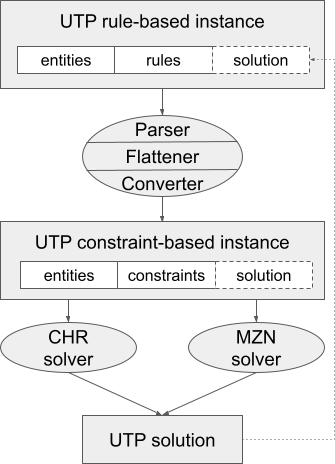
\includegraphics[scale=0.4]{img/utp_toolchain.png}
    \caption{The \UTP{} toolchain.}
    \label{fig:toolchain}
\end{figure}

Note that all constraints are handled as hard constraints and each {\UTP} instance is reduced to a hard constraint satisfaction problem ({\CSP}).
The ability to model preferences and multi-criteria objectives by the means of soft constraints is paramount in course timetabling and will be the subject of future extensions. 
Likewise, the catalog of {\UTP} predicates still lacks important constraints (e.g., gap, distribution and pattern constraints - see e.g. \cite{2017_aizam_AIPCP,2021_chen_IEEEA}) which will be gradually added in future versions.

As for implementation, the \UTP{} language is based on \XML{} and embedded in two constraint modeling languages, namely, 
{\MINIZINC} \cite{2007_nethercote_SPH,MINIZINC} and {\CHR} \cite{1994_fruhwirth_Chap}. 
We developed a tool chain consisting of a \XML{} parser, a rule processor to flatten rules into constraints, and an encoder to convert the resulting instances to solver-compatible formats %using {\JSON} or {\DZN}
(see Figure~\ref{fig:toolchain}). 
Beyond {\MINIZINC} and {\CHR}, constraint-based {\UTP} instances may be used as inputs to any solver implementing the model and predicates of the \UTP{} language.
We do not discuss here the \XML{} syntax of the language (the reader is referred to \cite{uspSite} which provides access to the detailed specification, %the {\JSON/\DZN} instance formats, 
%\cite{uspSite} also provides
the {\MINIZINC} and {\CHR} models, the tool suite, and a benchmark of instances).
Rather, we present the abstract syntax of the \UTP{} language and provide semantics for the key components.

The remainder of the paper is organized as follows.
Section~\ref{sec:schema} introduces the {\UTP} language and draws a comparison with %other modeling frameworks, notably 
the {\ITC} schema.
Section~\ref{sec:model} presents a generic constraint-based {\UTP} model.
Section~\ref{sec:cp-model} discusses its implementation using {\MINIZINC} and {\CHR}
and the cross-validation of the models on a real instance. 
Section~\ref{sec:conclusion} concludes and discusses extensions of this work.